\UC{Ricerca dei prodotti} 
L'utente non autenticato o l'acquirente può ricercare i prodotti dalla schermata principale oppure dalla \glo{PLP}.
\begin{itemize}
    \item \textbf{Attori primari:} acquirente o utente non autenticato;
    \item \textbf{Precondizione:} l'attore ha selezionato l'azione della ricerca e inserito le parole per la ricerca del prodotto;
    \item \textbf{Postcondizione:} l'attore viene spostato alla PLP con i prodotti che contengono almeno una delle parole ricercate nella descrizione o nel nome;
    \item \textbf{Scenario principale:} 
    \begin{itemize}
        \item L'attore inserisce le parole per la ricerca del prodotto;
        \item Preme sull'azione di ricerca;
        \item Viene portato alla PLP che contiene tutti i prodotti che hanno almeno una delle parole indicate nella descrizione o il titolo
    \end{itemize}
    \item \textbf{Estensioni:} l'utente ricerca dei prodotti non presenti nella piattaforma.
    \begin{itemize}
    	\item (\actualUC.1) - Visualizzazione messaggio di ricerca senza alcun risultato.
    \end{itemize}
\end{itemize}

\resetSubUC

\subUC{Visualizzazione messaggio di ricerca o filtraggio senza alcun risultato}
Nel caso in cui la ricerca o il filtraggio non dia risultati verrà visualizzato un opportuno messaggio.
\begin{itemize}
	\item \textbf{Attori primari:} acquirente, utente non autenticato;
	\item \textbf{Precondizione:} l'attore ha svolto una ricerca o un filtraggio che non ha prodotto alcun risultato;
	\item \textbf{Postcondizione:} all'attore verrà mostrato un messaggio che lo informa che la ricerca o il filtraggio non ha prodotto risultati;
	\item \textbf{Scenario principale:} l'attore effettua una ricerca o un filtraggio senza alcun risultato e viene avvertito.
\end{itemize}

\UC{Filtraggio prodotti della PLP}
\begin{figure}[H]
    \centering
    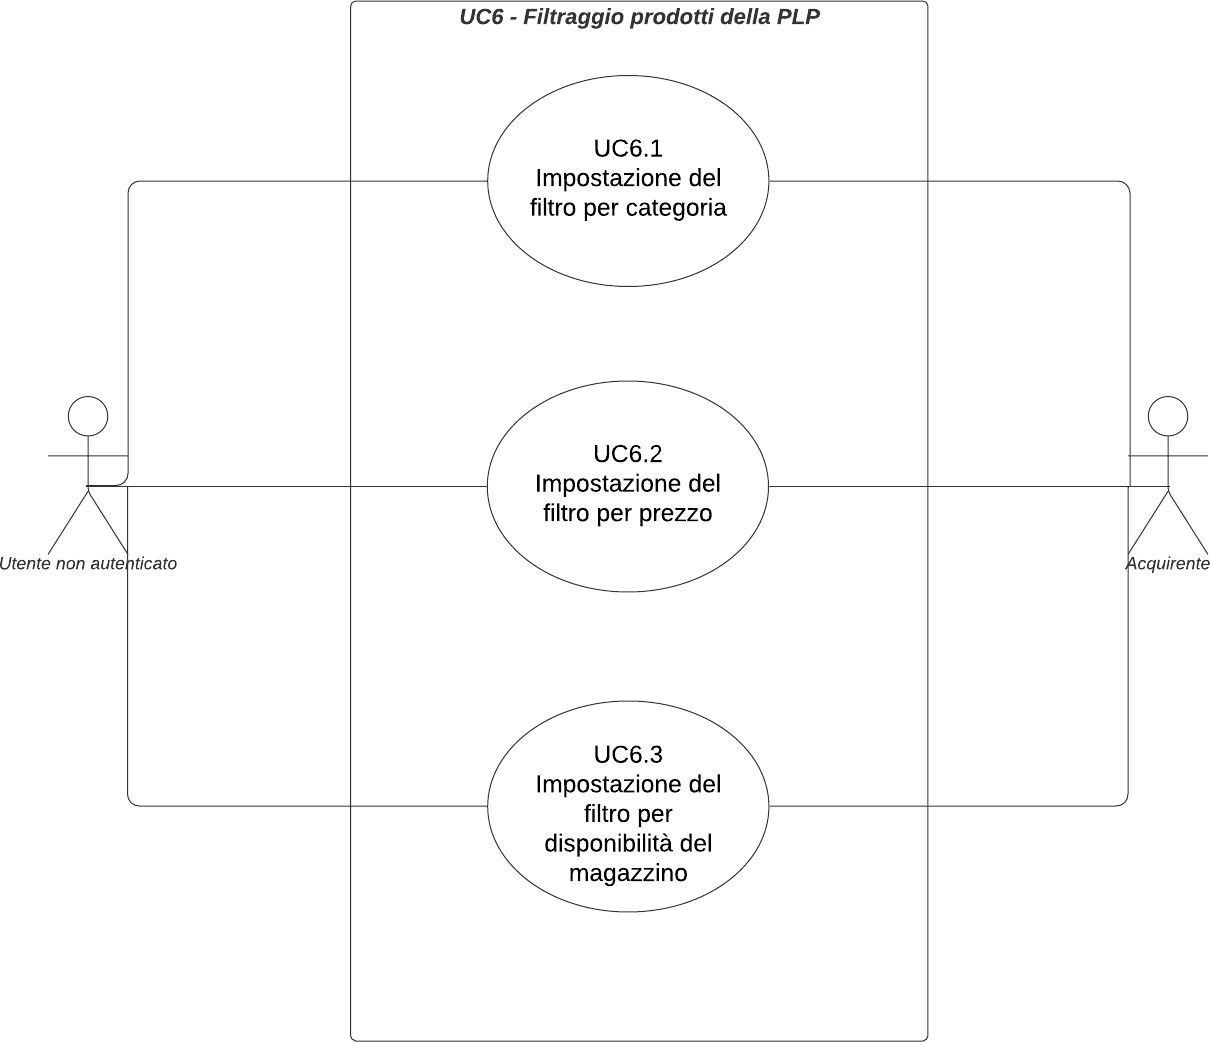
\includegraphics[scale=0.5]{Immagini/DiagrammiUC/UC6FiltraggioProdottiDellaPLP.png}
    \caption{Diagramma di \actualUC: Filtraggio dei prodotti della PLP} 
\end{figure}

L'utente non autenticato o l'acquirente filtra i prodotti all'interno della PLP in base alla categoria, per prezzo, per promozioni attive, sconti applicati e se c'è disponibilità nel magazzino.
\begin{itemize}
    \item \textbf{Attori Primari:} Acquirente; Utente non autenticato.
    \item \textbf{Precondizione:} L'attore è nella PLP e ha impostato uno (o più) dei filtri disponibili per i quali cercare.
    \item \textbf{Postcondizione:} L'attore avrà a disposizione tutti i prodotti che soddisfano tutte le condizioni dei vari filtri impostati.
    \item \textbf{Scenario Principale:}
    \begin{itemize}
        \item L'attore imposta uno (o più) dei filtri seguenti 
        \begin{itemize}
            \item (\actualUC.1) - Impostazione del filtro per categoria.
            \item (\actualUC.2) - Impostazione del filtro per prezzo.
            \item (\actualUC.3) - Impostazione del filtro per disponibilità nel magazzino.
        \end{itemize}
        \item La pagina viene aggiornata con i prodotti che rispettano i filtri applicati
    \end{itemize}
    \item \textbf{Estensioni:} Nel caso la combinazione di filtri impostati non dia risultati verrà visualizzato un messaggio dove viene segnalato all'attore questo fatto.
    \begin{itemize}
    	\item (UC) - Visualizzazione messaggio di ricerca o filtraggio senza alcun risultato.
    \end{itemize}
\end{itemize}

\resetSubUC

\subUC{Filtro per categorie}
L'utente non autenticato o l'acquirente può cercare i prodotti in base alla loro categoria, selezionando tra tutte le categorie disponibili.
\begin{itemize}
    \item \textbf{Attori Primari:} acquirente o utente non autenticato;
    \item \textbf{Precondizione:} l'attore è nella PLP e ha selezionato una (o più) categorie di quelle disponibili per quale filtrare;
    \item \textbf{Postcondizione:} l'attore avrà a disposizione i prodotti filtrati in base alle categorie selezionate;
    \item \textbf{Scenario principale:} l'attore seleziona le categorie per filtrare i prodotti.
\end{itemize}

\subUC{Filtro per prezzo}
L'utente non autenticato o l'acquirente può cercare i prodotti in base al loro prezzo.
\begin{itemize}
    \item \textbf{Attori Primari:} Acquirente; Utente non autenticato.
    \item \textbf{Precondizione:} L'attore è nella PLP e ha selezionato uno tra gli intervalli di prezzo disponibili (0 - 20, 20 - 50, 50 - 100, 100 - 200, 200 - 500, più di 500), oppure inserito un intervallo personalizzato.
    \item \textbf{Postcondizione:} L'attore avrà a disposizione i prodotti filtrati in base all'intervallo di prezzo selezionato.
    \item \textbf{Scenario Principale:} L'attore seleziona l'intervallo di prezzo oppure ne fornisce uno personalizzato per filtrare i prodotti.
\end{itemize}

\subUC{Filtro per disponibilità nel magazzino}
L'utente non autenticato o l'acquirente può cercare i prodotti in base alla loro disponibilità in magazzino.
\begin{itemize}
    \item \textbf{Attori Primari:} Acquirente; Utente non autenticato.
    \item \textbf{Precondizione:} L'attore è nella PLP e ha attivato il filtro per disponibilità in magazzino.
    \item \textbf{Postcondizione:} L'attore avrà a disposizione i prodotti che sono disponibili in magazzino.
    \item \textbf{Scenario Principale:} L'attore vuole visualizzare tutti i prodotti che sono disponibili in magazzino.
\end{itemize}
